\documentclass[12pt]{article}
\setlength{\oddsidemargin}{0in}
\setlength{\evensidemargin}{0in}
\setlength{\textwidth}{6.5in}
\setlength{\parindent}{0in}
\setlength{\parskip}{\baselineskip}

\usepackage{amsmath,amsfonts,amssymb,graphicx}

%\title{Review of Newtonian Mechanics}

\begin{document}

PHYS 374 Fall 2020\hfill Worksheet 2: Game of Fetch and the Principle of Least Time\\
\\
Name: \\
\\
Please submit as a PDF on Moodle. Include any calculations made using external tools.

\hrulefill
\\
\\
\noindent
Consider a game of fetch with a fluffy samoyed, Matoskah (``white bear" in Native American-Souian).
\begin{enumerate}
\item If Matoskah wants to collect a tennis ball on a flat playground in the shortest possible time, what is the best strategy?
\item If instead the tennis ball is thrown into a pond at location Y, shown in the diagram below, what time, $T$, does it take Matoskah to get to the tennis ball? State your final answer in terms of the various lengths stated in the diagram, $v_{1}$ and $v_{2}$. Make the following assumptions:
\begin{itemize}
\item Matoskah starts at $X$ and the tennis ball is floating at location $Y$.
\item Matoskah runs at a constant speed $v_{1}$, which is faster than the speed, $v_{2}$ at which he swims.
\item The shoreline is straight as shown.
\end{itemize}
\begin{figure}[h]
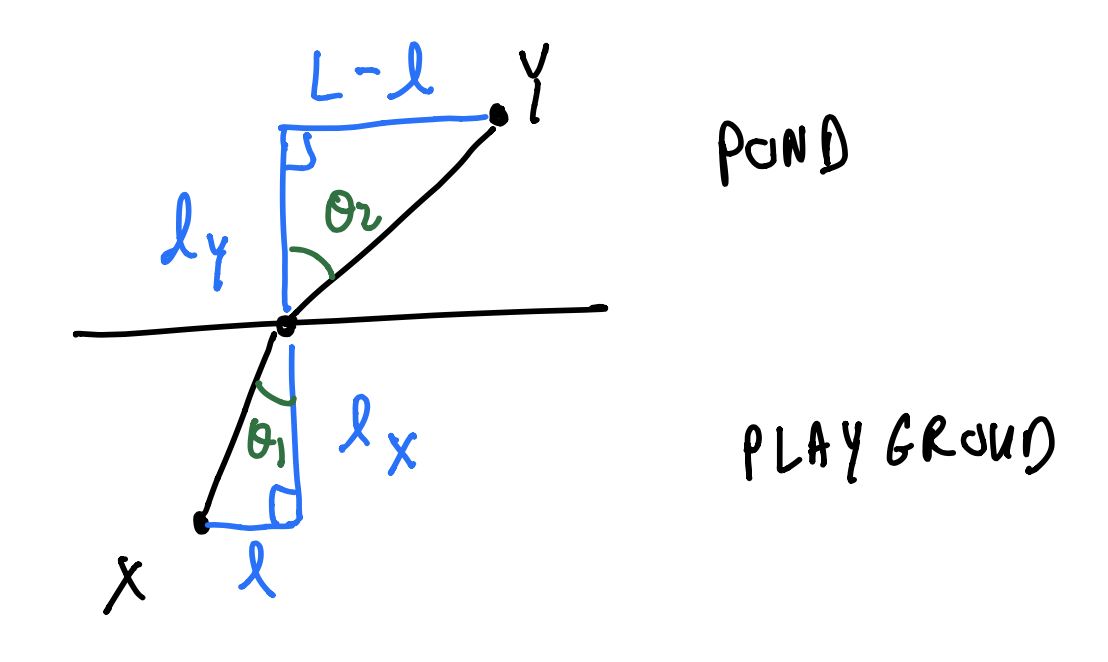
\includegraphics[width=8cm]{Diagram}
\centering
\end{figure}
\item Is the path shown in the diagram a good strategy to minimize the time? Discuss.
\item Find the path for which the time, $T$, is minimized stating your final answer in terms of $v_{1}$, $v_{2}$ and various lengths.
\item The index of refraction $n_{i}$ of medium $i$ is defined as $n_{i}=\frac{c}{v_{i}}$, where $c$ is the speed of light (and $n_{i}\ge 1$). Rewrite the time-minimizing condition of part 4. in terms of the indices of refraction of the playground, $n_{1}$, and that of the pond, $n_{2}$. Also, remove all lengths from the expression by using the angles $\theta_{1}$ and $\theta_{2}$.
\item Hypothesize a rule that light follows when propagating from one medium to another based on the results you have found.
\end{enumerate}
\end{document}